The dimension of the descriptor has a direct impact on the time it takes and less dimensions are desirable for fast interest point matching~\cite{Bay:08}. SIFT has 128 dimensional feature vector, which makes it very slow making it not suitable for real time applications. the high dimensionality of the descriptor is a drawback of SIFT at matching step. For online applications replying only on regular PC, each one of the three steps (detection, description, matching) has to be fast. Therefore, SURF method of feature detection has been developed to overcome the drawback of SIFT i.e. making matching algorithm faster by creation of low dimensional feature vector. \\

\noindent The SURF method can be described by the following two steps:\\
\begin{enumerate}
	\item \textbf{Interest Point Detection}
	\begin{itemize}
	    \item {\textit{Integral Images}} The computation time is reduced drastically by  using an intermediate representation of the image called \emph{integral image}~\cite{Viola:01}. The value at a location \textbf{X}=$(x,y)^T$ of integral image $II(\textbf{X})$ is calculated as:
	\begin{equation}
	II(\textbf{X})=\sum_{i=0}^{i \leq x}{\sum_{j=0}^{j\leq y}{I(i,j)}}
	\label{eq:integral-image}
	\end{equation}
	After computing of integral image, we can calculate the intensity of any vertical rectangle as shown in figure~\ref{fig:intensity-calculation}. The calculation time is independent of the the size.
	
	\begin{figure}[H]%
	\centering
	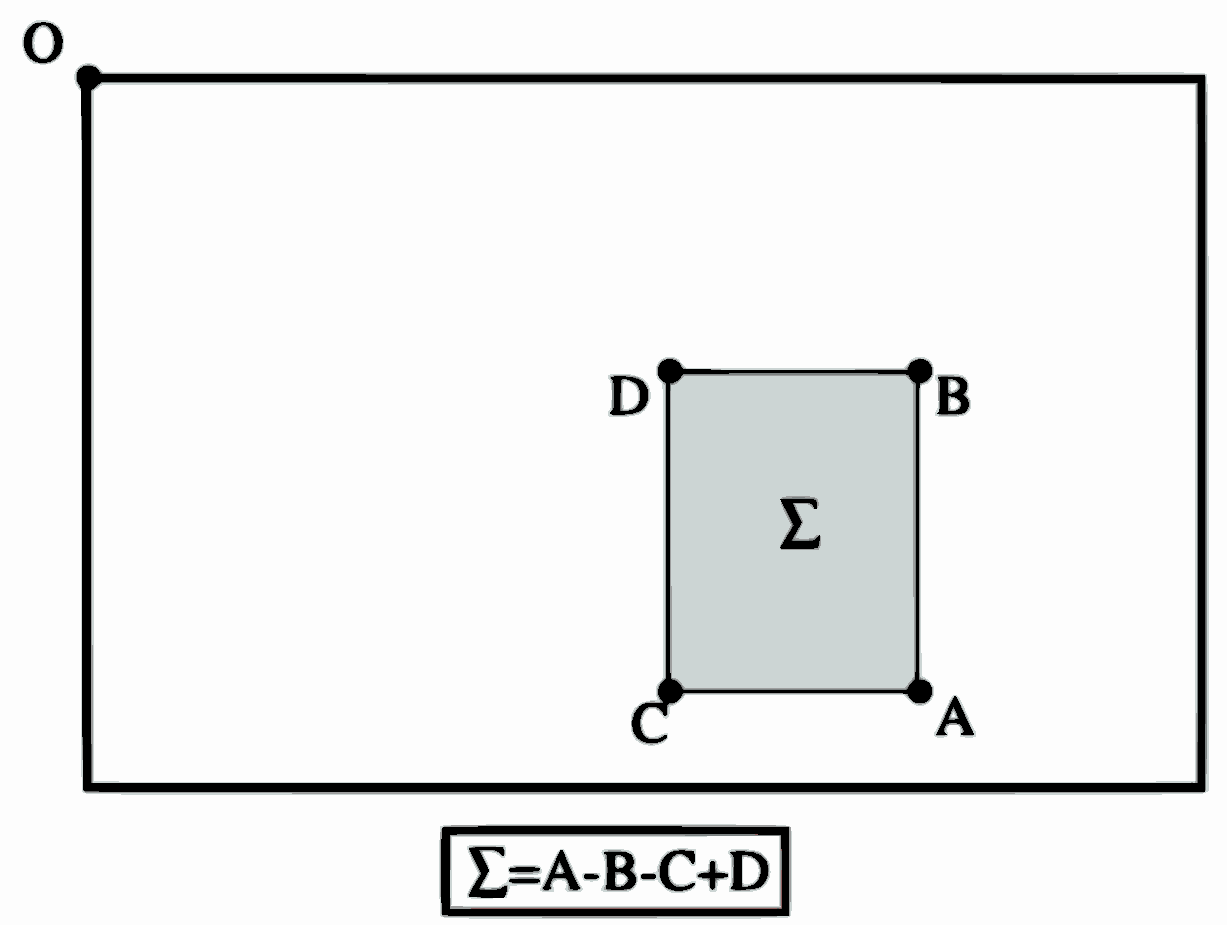
\includegraphics[width=0.6\columnwidth]{2.mainmatter/2.Methodology/FeaturesExtraction/figures/SURF/intensity-calculation}%
	\caption[Calculation of Sum of Intensities]{Calculation of sum of intensities inside a rectangular region of integral image. \imgsrc{(Image source: Bay \emph{et al}~\cite{Bay:08})}}%
	\label{fig:intensity-calculation}%
	\end{figure}
	\item {\textit{Hessian matrix}} For any point \textbf{x} = (x,y) in image $I$, the Hessian matrix $H(x,\sigma)$ can be defined as:\\
	\begin{equation}
  H(x,\sigma)=\left[ \begin{array}{cc}
	L_{xx}(x,\sigma) & L_{xy}(x,\sigma)\\
	L_{xy}(x,\sigma) & L_{yy}(x,\sigma)	
\end{array}
\right]
\label{eq:hess-matrix}
\end{equation}
where
\begin{equation} L_{xx}(x,\sigma)=\frac{\partial^2}{\partial_x^2}g(\sigma)\otimes I
\label{eq:Lxx}
\end{equation}

\begin{equation}
L_{yy}(x,\sigma)=\frac{\partial^2}{\partial_y^2}g(\sigma)\otimes I
\label{eq:Lyy}
\end{equation}


\begin{equation}
L_{xy}(x,\sigma)= \frac{\partial^2}{\partial_x \partial_y}g(\sigma) \otimes I
\label{eq:Lxy}
\end{equation}
The Gaussian functions are discretized and cropped, so there is some loss of repeatability of Hessian based detectors under image rotations; but this is out-weighted by the advantage of fast convolution by the descretization and cropping~\cite{Bay:08}. The approximated determinant of Hessian matrix represents the blob response in the image at location \textbf{x}. Bay \emph{et al.}\cite{Bay:08} suggests to use 9x9 box filters as shown in figure~\ref{fig:approx-gaussian-partial} to create the blob responses $D_{xx}$, $D_{yy}$, $D_{xy}$. Then computation of determinant of Hessian i.e. $det(H_{approx})$ is computed as follows:
\begin{equation}
det(H_{approx})=D_{xx}D_{yy}-w(D_{xy}^2)
\label{eq:det-hessian-apprx}
\end{equation}
here, w is used to balance the expression for the Hessian's determinant. Generally, it does not have a significant impact on the result, so we keep this value as constant\cite{Bay:08}. \\

\begin{figure}[H]%
\centering
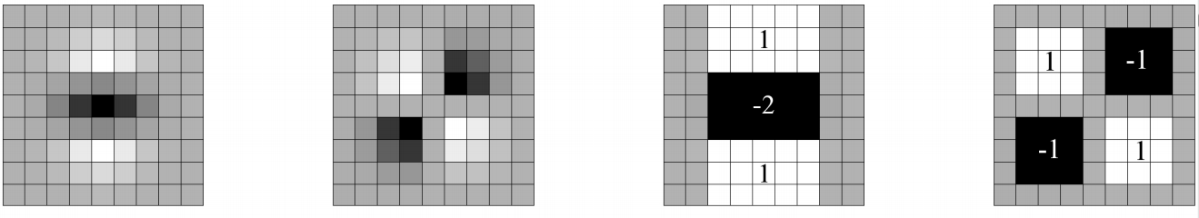
\includegraphics[width=\columnwidth]{2.mainmatter/2.Methodology/FeaturesExtraction/figures/SURF/approx-gaussian-partial}%
\caption[Approximation of Gaussian Partial Derivative]{Left two images are cropped and decretized Gaussian second order partial derivative ($L_{yy}$, $L_{xy}$), right two images are corresponding approximated filters ($D_{yy}$, $D_{xy}$).}%
\label{fig:approx-gaussian-partial}%
\end{figure}
\item{\textit{Scale Space Representation}}
\noindent The scale space is analyzed by up-scaling the box filter size rather than iteratively reducing the image size (figure~\ref{fig:upscaling}). The output of the 9 x 9 filter is the initial scale layer (scale=1.2, because the approximation was with $\sigma$=1.2). By doing this, we achieve computational efficiency and there will be no aliasing because we don't need to down-sample the image~\cite{Bay:08}.\\


\begin{figure}%
\centering
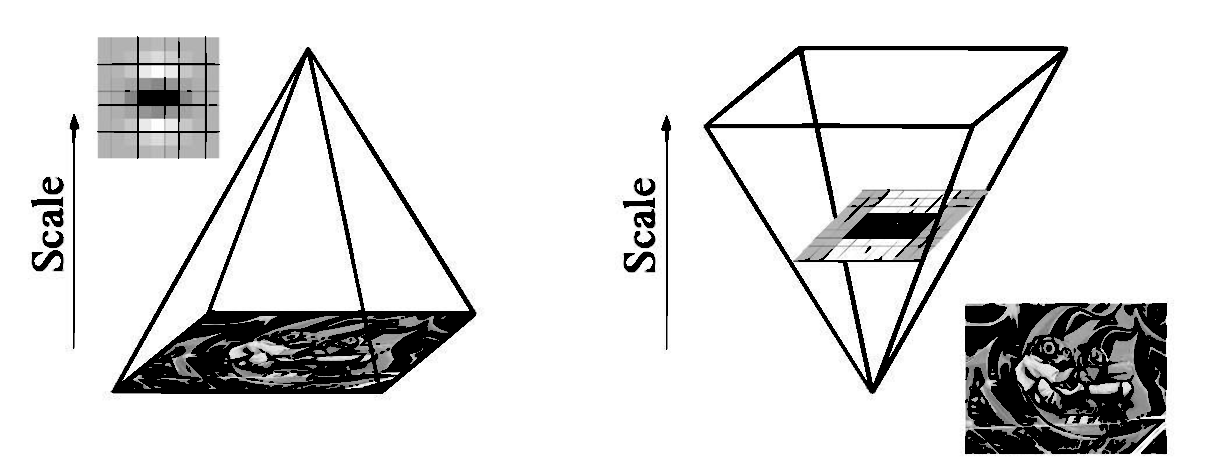
\includegraphics[width=\columnwidth]{2.mainmatter/2.Methodology/FeaturesExtraction/figures/SURF/upscaling-integral}%
\caption[Scale Space Generation]{The use of integral images allows up-scaling of the filter at constant cost.}%
\label{fig:upscaling}%
\end{figure}

\noindent The scale space is divide into octaves. An octave represents a series of filter response maps obtained by convolving the same input image with a filter of increasing size. Each octave is divided into a constant number of scale levels as shown in figure~\ref{fig:filters-octaves}

\begin{figure}[H]%
\centering
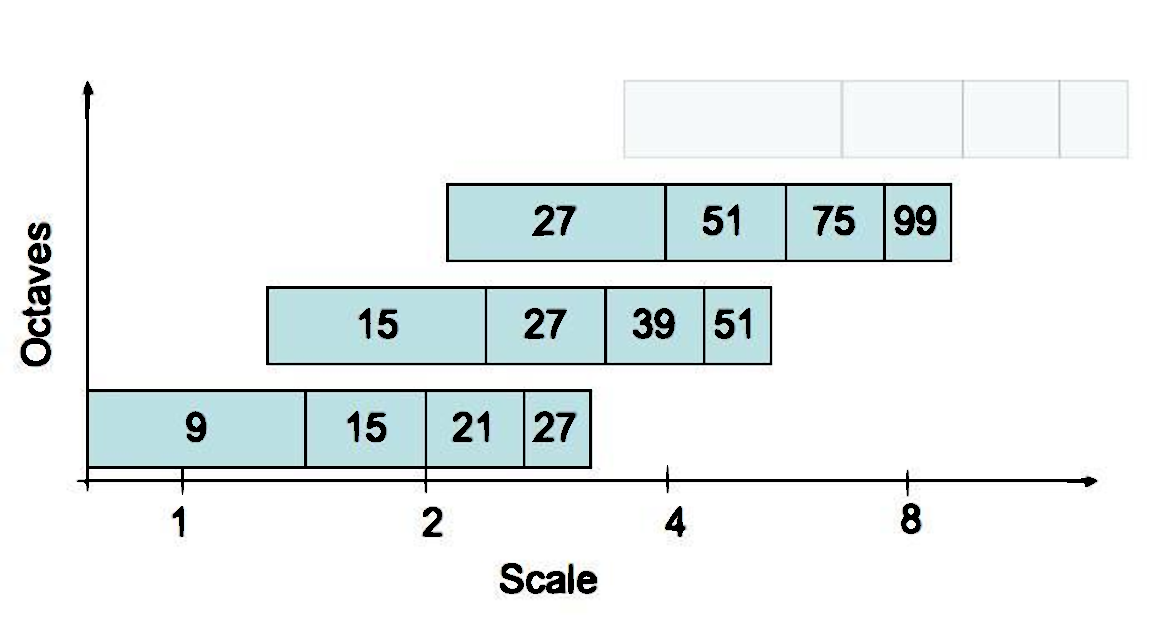
\includegraphics[width=0.6\columnwidth]{2.mainmatter/2.Methodology/FeaturesExtraction/figures/SURF/octaves-scales}%
\caption[Scaling in Octaves]{Filter side lengths for three different octaves. \imgsrc{(Image source: Bay \emph{et al}~\cite{Bay:08})}}%
\label{fig:filters-octaves}%
\end{figure}

\item {\textit{Interest Point Localization}}
After successful, scale-space creation, the next task is to localize the interest points.To localize interest points in the image and over scales, a non-maximum suppression in a 3 x 3 x 3 neighborhood is applied. The maxima of the determinant of the Hessian matrix are then interpolated in scale and image space.\cite{Bay:08}.
\end{itemize} 
	
\item \textbf{Interest Point Description} The method of descriptor extraction is similar to SIFT described in previous section. The distribution of first order Haar wavelet responses in x and y direction (figure~\ref{fig:haar-wavelets}) instead of the gradient is used for descriptor extraction. We exploit integral images for speed. The use of only 64 dimensional feature vector greatly reduces the time for matching while increasing the robustness~\cite{Bay:08}. The authors of SURF claims the new indexing step based on the sign of the Laplacian increases the robustness of the descriptor and matching speed also; so the name SURF-Speeded-Up Robust Features.\\

\begin{figure}[H]%
\centering
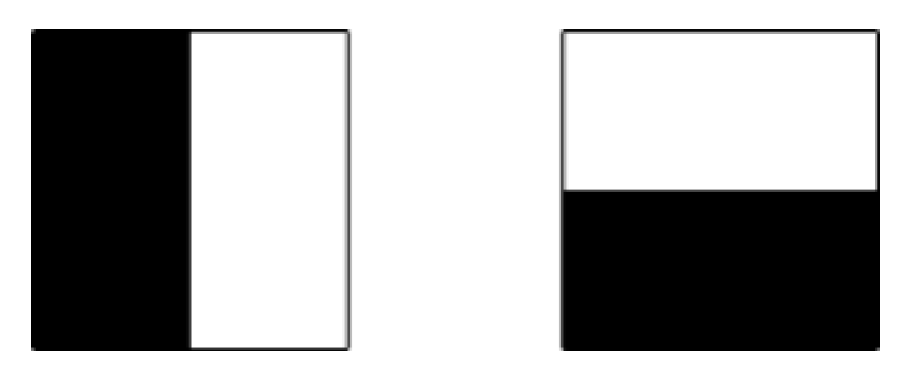
\includegraphics[width=\columnwidth]{2.mainmatter/2.Methodology/FeaturesExtraction/figures/SURF/haar-wavelets}%
\caption[Haar Wavelets]{Haar Wavelets: The left one is response in x-direction, the right one is response in y-direction. Weight=1 for black region, -1 for white region. \imgsrc{(Image source: Evans~\cite{Evans:09})}}%
\label{fig:haar-wavelets}%
\end{figure}


The interest points descriptors are assigned by the following two steps:
\begin{itemize}
	\item {\textit{Orientation Assignment}} Orientation assignment is carried out for rotation invariance. Haar wavelet responses of size 4$\sigma$ are calculated for a set of pixels within a radius of 6$\sigma$ of detected point.\footnote{$\sigma$ is the scale at which the point was detected.} The specific set of pixels is determined by sampling those from within the circle using step size of $\sigma$~\cite{Evans:09}. Weighted responses with a Gaussian centered at the interest point are used to find the dominant orientation in each circle segment of angle $\frac{\pi}{3}$ (i.e. 60\deg) around the origin. At each position, the x and y- responses within the segment are summed and used to form a new vector. The longest vector is the orientation of the interest point~\cite{Evans:09}.This process is shown in figure~\ref{fig:orientation-assignment}.
	
	
	\begin{figure}[H]%
	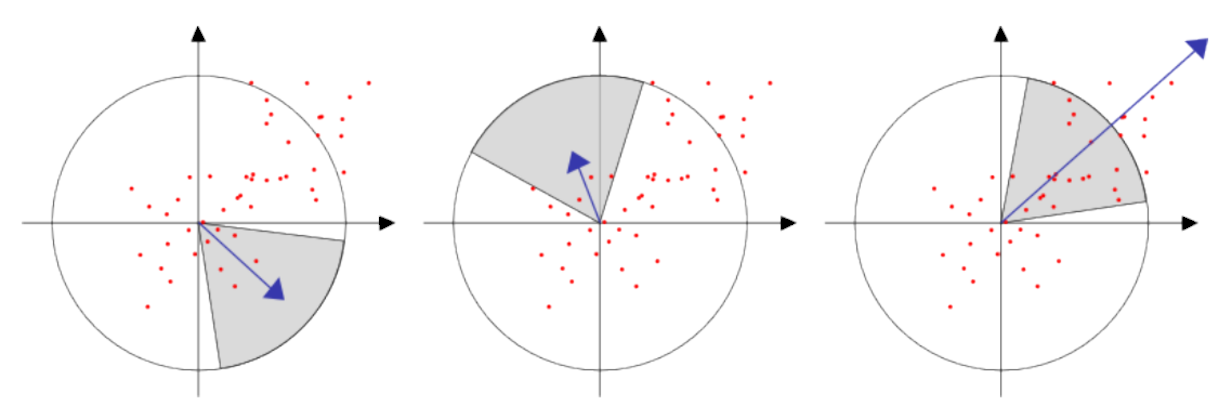
\includegraphics[width=\columnwidth]{2.mainmatter/2.Methodology/FeaturesExtraction/figures/SURF/orientation-assignment}%
	\caption[Orientation Assignment]{Orientation Assignment: The blue arrow is the sum of the responses. The largest one determines the dominant orientation. \imgsrc{(Image source: Evans~\cite{Evans:09})}}%
	\label{fig:orientation-assignment}%
	\end{figure}	
	
	\item{\textit{Descriptor Components}} We construct a square window of size 20$\sigma$ around the interest point. The orientation of the window will be the dominant orientation we calculated above. This descriptor window is divided into 4 x 4 regular sub-regions. We select 25 regularly distributed sample points in each sub-region and Haar wavelets of size 2$\sigma$ are calculated for those points~\cite{Evans:09}. Then, the feature vector for each sub-region will be
	\begin{equation}
	V_{subregion}=\left[ \Sigma dx,\Sigma dy,\Sigma \left| dx \right|,\Sigma \left| dy\right| \right]
	\label{eq:feature-vector}
	\end{equation}
	
	
As shown in figure~\ref{fig:descriptor-components}, each sub-region will have four values to the descriptor vector which results the overall vector length 4 x 4 x 4=64. Evans in his article~\cite{Evans:09} claims that the result SURF descriptor is invariant to rotation, scale, brightness and contrast\footnote{invariant to contrast is achieved after reduction to unit length~\cite{Evans:09}.}.
\begin{figure}[H]%
	   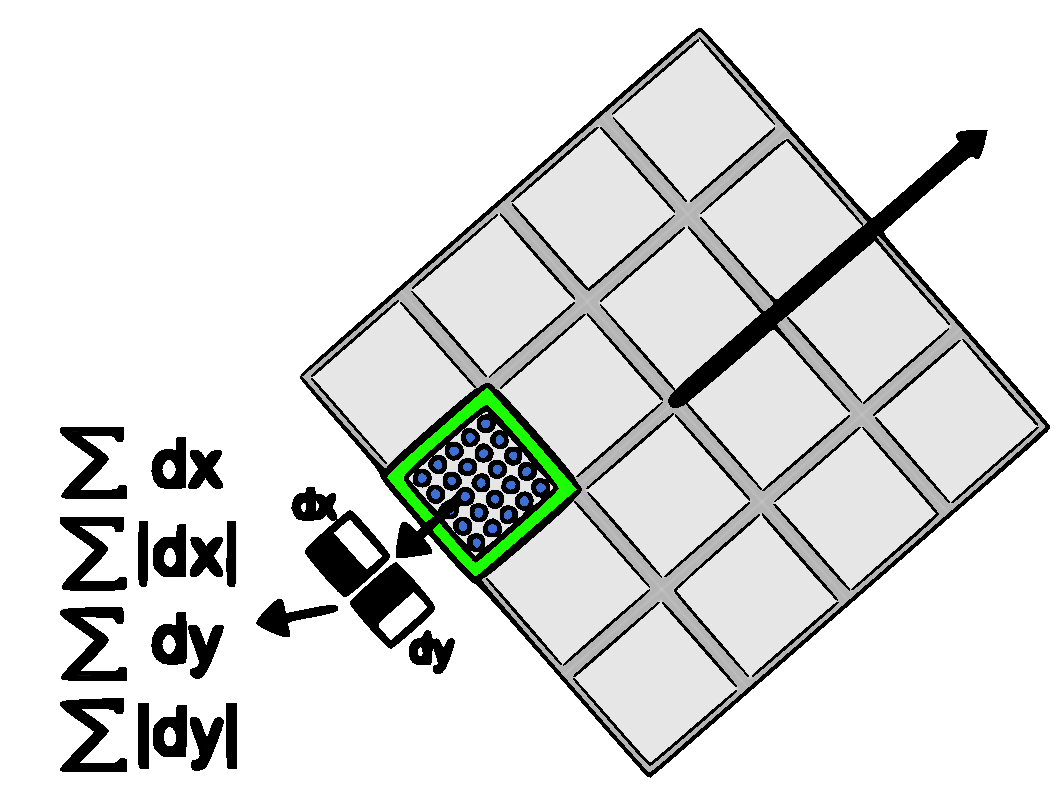
\includegraphics[width=\columnwidth]{2.mainmatter/2.Methodology/FeaturesExtraction/figures/SURF/descriptor-components}%
	   \caption[Descriptor Components]{Descriptor Components.  \imgsrc{(Image source: Evans~\cite{Evans:09})}}%
	   \label{fig:descriptor-components}%
\end{figure}	
	
	
\end{itemize}


\end{enumerate}